The Java Runtime Environment (JRE) is the collection of all the software and utilities needed to run compiled Java programs, basically it is composed by the JVM (Java Virtual Machine) and the JCL (Java Class Library, the Java API).
The reference documentation for the Java programming language can be found \href{https://docs.oracle.com/javase/specs/index.html}{here}.

\section{JVM internals}
The JVM is an abstract machine whose machine language is the Java bytecode.
The java specification does \emph{not} give implementations details like memory layout of run-time data area, garbage collection algorithm, internal optimization and more but defines a machine independent \emph{class file format} that all JVM implementations must support.
Moreover the JVM imposes strong syntactic and structural constraints on the code in a class file, so that any language with functionality that can be expressed in terms of a valid class file can be hosted by the JVM.

\subsection{Execution model}
The JVM is a multi-threaded stack based machine, it means that the JVM instructions implicitly take arguments from the top of the operand stack of the current frame and put their result on top of it.

So the operand stack is used to:
\begin{itemize}
    \item pass arguments to methods;
    \item return a result from a method;
    \item store intermediate results while evaluating expressions;
    \item store local variables.
\end{itemize}

It's abstract machine hierarchy is:
\begin{figure}[H]
    \centering
    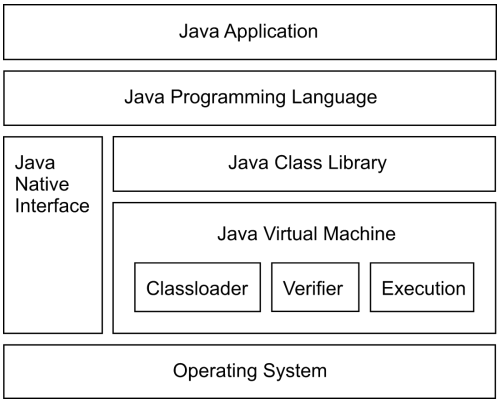
\includegraphics[width=250px]{images/2_JVM/JVM_hierarchy.png}
    \caption{JVM hierarchy}
\end{figure}

\subsection{Class files}
A class file is a file which holds the external representation of the code and data of a program and is platform independent (it's in fact standardized in the java docs).
Once the file is loaded by a JVM we get the internal representation which is strongly tied with the JVM implementation, so it's implementation dependent.

\subsection{Data Types}
The JVM provides common primitive types:
\begin{itemize}
    \item numeric integral: byte, short, int, long, char;
    \item numeric floating point: float, double;
    \item boolean;
    \item internal types for exception handling: returnAddress.
\end{itemize}
and some more reference types:
\begin{itemize}
    \item class types;
    \item array types;
    \item interface types.
\end{itemize}

It is important to note that at run-time on local variable there is no information regarding the type because the type of the operand is already specified by the used opcodes (for example using \verb|iadd| we are implicitly saying that operands are integer whether with \verb|fadd| we are referring to floating point numbers).

The representation of the objects is left to the implementation, the concrete value of \verb|null| too.
It is added an extra level of indirection because pointers to instances and class attributes are used, it makes the garbage collection easier.
An important specification for the object representation is the inclusion of a mutex lock and some flags for the garbage collection state.

\subsection{Threads}
JVM allocates multiple threads per application starting with main.
They can be created instantiating the \verb|Thread| class (or class that inherits from it or implement \verb|Runnable|) and calling the \verb|start| method (which invokes \verb|run|).
Moreover there are some system threads (namely daemon threads) for garbage collection, object finalization, signal dispatching, compilation, ecc.
Threads can be supported both via time-slicing and multiple processors.

Regarding the memory all the threads can access the heap and the persistent memory and each thread has a per-thread area in which resides the stack for that thread.

\begin{figure}[H]
    \centering
    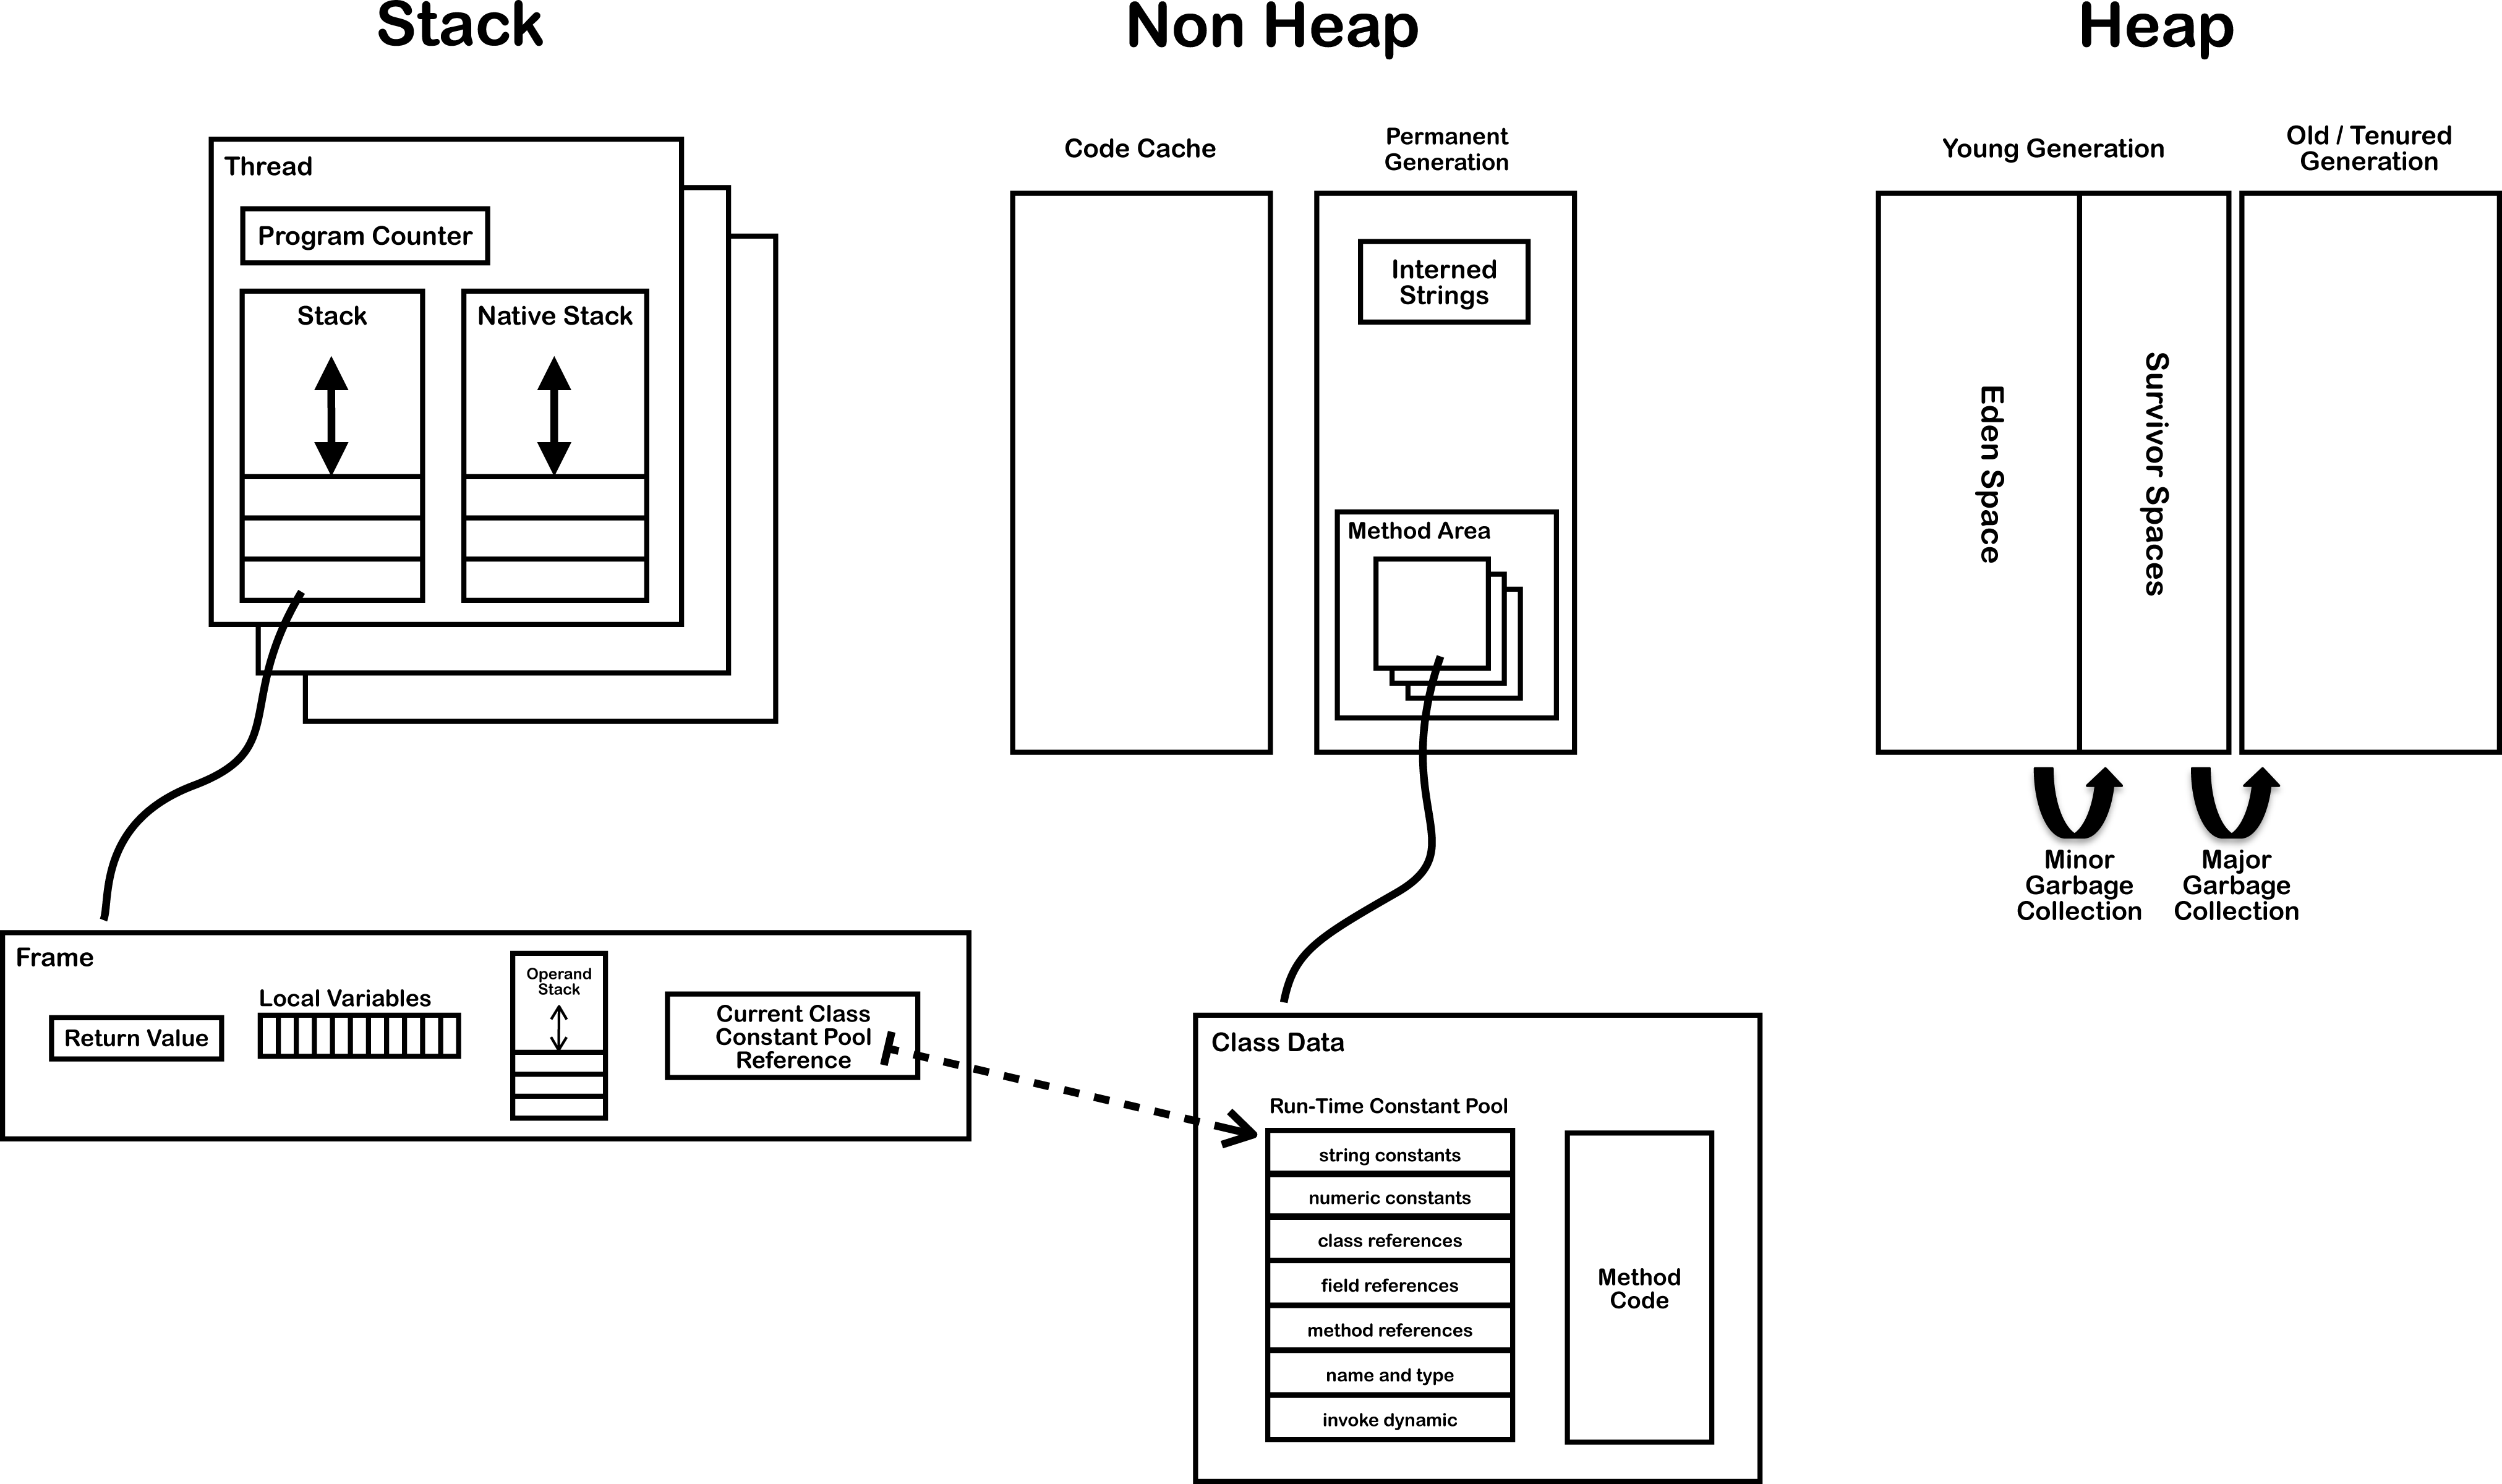
\includegraphics[width=400px]{images/2_JVM/JVM_Internal_Architecture.png}
    \caption{JVM internal architecture}
\end{figure}
There are some complex specification for the consistency model in the language specification.

\subsection{Per Thread Data Areas}
Each thread must hold:
\begin{itemize}
    \item \verb|pc|: a pointer to the next instruction to execute, inside the method area.
    It's value is undefined if the current method is \emph{native}.
    
    \item the java stack: is a stack of frames (activation records).
    A new frame is created each time a method is invoked and it is destroyed when the method completes and returns.
    Frames doesn't necessarily must be allocated contiguously.
    
    \item the native stack: it is used for the invocation of native functions through the JNI (Java Native Interface).
    When a native function is invoked the execution continues using this native stack in order to isolate the JVM environment from the outside and allow communication between the two worlds only via JNI.
    It's also a security feature.
\end{itemize}

\subsubsection{Structure of frames}
Each frame contains:
\begin{itemize}
    \item local variable array: array of 32 bits elements containing a reference to \verb|this| (if it's an instance method), method parameters and then local variables;

    \item operand stack: a stack used in evaluation of expressions and evaluation of the method, this is the stack manipulated by the JVM instructions;
    
    \item a reference to the Constant Pool of the current class.
\end{itemize}

\subsubsection{Constant Pool and Dynamic linking}
In C/C++ multiple objects file are linked together to produce a executable or a shared library, so all those objects file are joined together and the symbolic references are replaced with an actual memory address relative to the final executable.
In Java this linking phase is done dynamically at run-time, during the compilation in fact all references to variables and methods are stored in the class's constant pool as symbolic references, then the JVM can resolve those symbolic references using:
\begin{itemize}
    \item eager or static resolution: when the class file is verified after being loaded;
    \item lazy or late resolution: when the symbolic reference is used for the first time.
\end{itemize}
but the JVM has to behave lazily so the errors must be thrown at the first usage of the faulty reference.

The resolution happens only once because the symbolic reference is completely replaced in the constant pool by its result, this process is called \emph{binding}.

If the symbolic reference refers to a class that has not yet been resolved then this class will be loaded, so the constant pool reference inside the stack frame helps a lot during this dynamic linking mechanism.

\subsection{Shared by threads Data Areas}
Those structures are divided in:
\begin{itemize}
    \item heap: in which resides the objects and the arrays.
    The explicit de-allocation from heap is not supported, only the garbage collection can reclaim occupied memory.
    The HotSpot JVM (the oracle one) includes four Generational Garbage Collection Algorithms which became Z Garbage collector since oracle JDK 11.
    
    \item non-heap: in which resides objects which are never de-allocated and there are the structures who are needed for the JVM execution like method area, interned strings and the code cache for JIT.
\end{itemize}

\subsubsection{JIT}
Some JVMs profiles the code during the interpretation in order to find the areas which are executed regularly, those parts are then compiled to native code in order to be faster during the next executions.
Such produced code is stored in the code cache in non-heap area.

\subsection{Class File structure}
The structure of the class file is the following:
\begin{figure}[H]
    \centering
    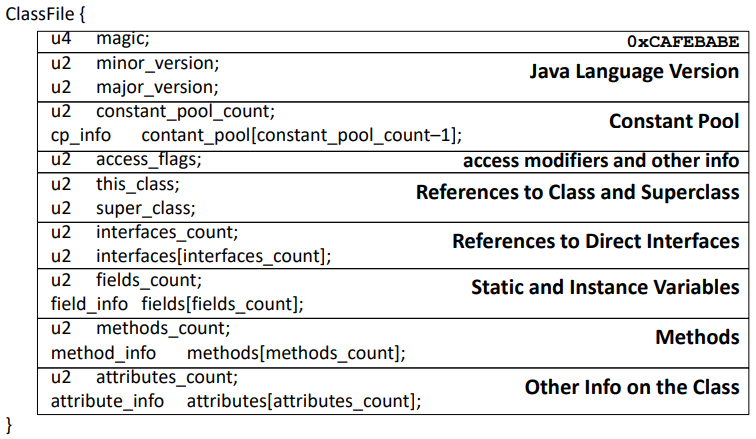
\includegraphics[width=350px]{images/2_JVM/class_file_structure.png}
    \caption{Class file structure}
\end{figure}

\subsection{Method Area}
This memory region holds class file when are loaded, for each class then are stored:
\begin{itemize}
    \item a reference to the Classloader;
    \item Run Time Constant Pool;
    \item Field Data;
    \item Method data;
    \item Method code.
\end{itemize}
We said that non-heap area is shared among threads, so the access must be thread safe during the updates in this region which are only class loading and symbolic link resolving.

Each field of the method area has some data:
\begin{itemize}
    \item a name;
    \item a type: a descriptor which says the type of the field, according to the following table:
    \begin{figure}[H]
        \centering
        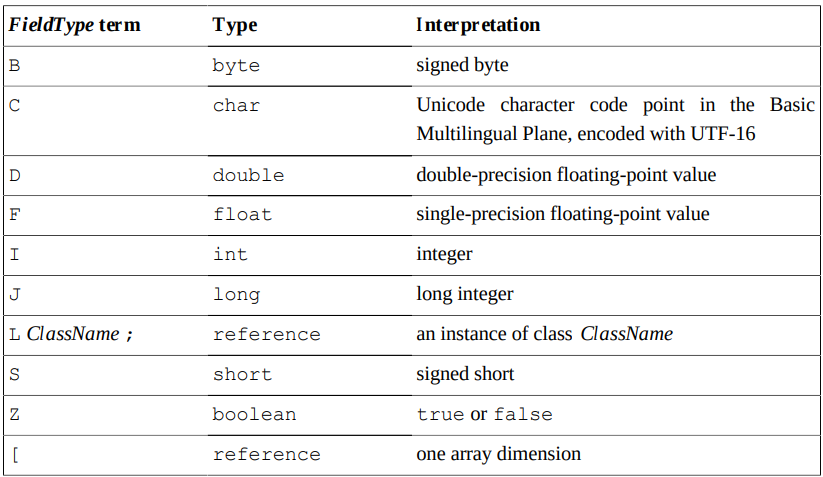
\includegraphics[width=350px]{images/2_JVM/fieldtype_descriptors.png}
        \caption{FieldType descriptors}
    \end{figure}
    \item some modifiers;
    \item some attributes.
\end{itemize}

Each method encodes all the necessary information like:
\begin{itemize}
    \item name;
    \item return type;
    \item parameter types (in the specified order);
    \item modifiers;
    \item attributes;
    \item the code.
\end{itemize}
The method descriptor contains the sequence of the parameter descriptors in brackets and the return descriptor (or \verb|V| for void), for example: \verb|Object m(int i, double d, Thread t){...}| gets translated in \verb|(IDLjava/lang/Thread;)Ljava/lang/Object;| (\verb|I| for the int parameter, \verb|D| for the double parameter, \verb|Ljava/lang/Thread;| for the Thread parameter and \verb|Ljava/lang/Object;| for the Object return type).


Each method then stores:
\begin{itemize}
    \item the bytecode of the actual code;
    \item operand stack size;
    \item local variable size;
    \item local variable table;
    \item exception table;
    \item LineNumberTable: tells which line of source code corresponds to which byte code instruction, it is used for debugging;
    \item some exception handling information, one for each try/catch/finally clause, like:
    \begin{itemize}
        \item start point;
        \item end point;
        \item program counter offset for handler code;
        \item constant pool index for exception class being caught.
    \end{itemize}
\end{itemize}

\subsection{Tools}
The JDK (Java Development Kit) gives us some useful tools to compile, disassemble and execute java executables:
\begin{itemize}
    \item \verb|javac|: is the java compiler, it takes source code and gives us valid class files;
    \begin{verbatim}
        $ javac SimpleClass.java
        # produces SimpleClass.class
    \end{verbatim}
    \item \verb|javap|: is the java disassembler, disassembled the java bytecode in human readable format;
    \begin{verbatim}
        $ javap -c -v SimpleClass.class
    \end{verbatim}
    \item \verb|java|: is the actual JVM in charge of executing the bytecode.
    \begin{verbatim}
        $ java SimpleClass
    \end{verbatim}
\end{itemize}

\subsection{Let's analyze a disassembled example class}
Let's compile the following code:
\begin{verbatim}
    package org.jvminternals;
    public class SimpleClass {
        public void sayHello() {
            System.out.println("Hello");
    }}
\end{verbatim}
it's disassembled version is:
\begin{verbatim}
{
    public org.jvminternals.SimpleClass();
        descriptor: ()V
        flags: ACC_PUBLIC
        Code:
            stack=1, locals=1, args_size=1
                0: aload_0
                1: invokespecial #1 // Method java/lang/Object."<init>":()V
                4: return
            LineNumberTable:
                line 2: 0

    public void sayHello();
        descriptor: ()V
        flags: ACC_PUBLIC
        Code:
            stack=2, locals=1, args_size=1
                0: getstatic #2 // Field java/lang/System.out:
                    //Ljava/io/PrintStream;
                3: ldc #3 // String Hello
                5: invokevirtual #4 // Method 
                    // java/io/PrintStream.println:(Ljava/lang/String;)V
                8: return
            LineNumberTable:
                line 4: 0
                line 5: 8
}
SourceFile: "SimpleClass.java”
\end{verbatim}
Something to notice:
\begin{itemize}
    \item \verb|()V|: in the descriptor sections are the method descriptors, in fact both methods (a default constructor and the method \verb|sayHello|) take zero arguments and return nothing, so type void;
    \item \verb|invokespecial #1|: is the index of the method to invoke inside the constant pool;
    \item \verb|aload_0|: says to load the element at position 0 in the local variables array, which is the \verb|this| reference;
    \item \verb|Field java/lang/System.out:Ljava/io/PrintStream;|: is the resolution of the field descriptor which the \verb|#2| points to;
    \item \verb|String Hello|: is the string literal to which \verb|#3| points to.
\end{itemize}

\subsubsection{Constant Pool}
A constant pool is similar to a symbol table but it holds more info.
Basically it contains constants and symbolic references used for dynamic binding with of course tags for the underlying type of the value:
\begin{itemize}
    \item numeric literal;
    \item string literal;
    \item class reference;
    \item field references;
    \item method references (\verb|Methodref|, \verb|InterfaceMethodref|, \verb|MethodHandle|);
    \item signatures (Name and types);
\end{itemize}
So operands in the bytecode are often indexes in the constant pool.

An example of constant pool is (always from the previous disassembled file):
\begin{verbatim}
Compiled from "SimpleClass.java"
    public class SimpleClass
    minor version: 0
    major version: 52
    flags: ACC_PUBLIC, ACC_SUPER
Constant pool:
    #1 = Methodref #6.#14 // java/lang/Object."<init>":()V
    #2 = Fieldref #15.#16 // java/lang/System.out:Ljava/io/PrintStream;
    #3 = String #17 // Hello
    #4 = Methodref #18.#19 // java/io/PrintStream.println:(Ljava/lang/String;)V
    #5 = Class #20 // SimpleClass
    #6 = Class #21 // java/lang/Object
    #7 = Utf8 <init>
    #8 = Utf8 ()V
    #9 = Utf8 Code
    #10 = Utf8 LineNumberTable
    #11 = Utf8 sayHello
    #12 = Utf8 SourceFile
    #13 = Utf8 SimpleClass.java
    #14 = NameAndType #7:#8 // "<init>":()V
    #15 = Class #22 // java/lang/System
    #16 = NameAndType #23:#24 // out:Ljava/io/PrintStream;
    #17 = Utf8 Hello
    #18 = Class #25 // java/io/PrintStream
    #19 = NameAndType #26:#27 // println:(Ljava/lang/String;)V
    #20 = Utf8 SimpleClass
    #21 = Utf8 java/lang/Object
    #22 = Utf8 java/lang/System
    #23 = Utf8 out
    #24 = Utf8 Ljava/io/PrintStream;
    #25 = Utf8 java/io/PrintStream
    #26 = Utf8 println
    #27 = Utf8 (Ljava/lang/String;)V
\end{verbatim}

So basically the \verb|sayHello| function does:
\begin{itemize}
    \item \verb|getstatic #2|: fetches the operand \verb|java/lang/System.out:Ljava/io/PrintStream| \\
    and pushes it onto the operand stack;
    \item \verb|ldc #3|: fetches the string \verb|Hello| and pushes it onto the operand stack;
    \item \verb|invokevirtual #4|: calls \verb|java/io/PrintStream.println:(Ljava/lang/String;)V| \\
    which takes the arguments from the operand stack and executes the print function.
\end{itemize}

\subsection{Run-time constant pool}
The constant pool inside the class file is used to construct the run-time constant pool.
All references in the run-time pool are initially symbolic then are resolved at the first access in the expected way.
Class names are the ones returned by \verb|Class.getName()| and the field and method references are made of name, descriptor and class name.

\section{JVM life cycle}
The JVM starts up by loading an initial class using the \emph{bootstrap classloader}.
Loading means: finding the binary representation of a class or interface type with a given name and creating a class or interface from it.
Then that class is linked: the class file content is combined into the run-time state of the JVM, then it's initialized: so the initialization method \verb|<clinit>| is called.
Then the function \verb|public static void main(String [])| is invoked which will trigger the loading, linking and initialization of additional classes and interfaces.

\subsection{More on loading}
The creation of a class or an interface is triggered by someone referencing it or by certain methods (the ones who are used for reflection).
The JVM of course checks if the class has already been loaded, if not it is invoked the \verb|loadClass| method from the loader class specified in the class file, then each class is tagged with the \emph{initiating loader} and the \emph{loading constraints} are checked during loading to ensure that the same name denotes the same type in different loaders.

\subsubsection{Class loader hierarchy}
There exists a proper hierarchy among the different class loaders:
\begin{itemize}
    \item Bootstrap classloader: it loads basic Java APIs and may skip some of the validations that should be done for the normal classes;
    \item Extension classloader: it loads classes from standard Java extension APIs such as security extensions functions;
    \item System classloader: it is the default one;
    \item User defined classloader: can be used to load application classes:
    \begin{itemize}
        \item for runtime reloading of classes;
        \item for loading from different sources (network, encrypted file, or on the fly generation);
        \item for supporting separation between different groups of loaded classes as required by web servers;
    \end{itemize}
\end{itemize}
The basic classloader interface is composed by:
\begin{itemize}
    \item \verb|findClass|: which builds an array of bytes;
    \item \verb|defineClass|: which turns an array of bytes into a class object;
    \item \verb|resolveClass|: which links a class.
\end{itemize}

\subsection{More on Linking}
Linking is made by 3 main phases:
\begin{itemize}
    \item verification: it is actually made both during the load and the link process.
    That phase is important because there is no guarantee that the class file was generated correctly by a java compiler, nor that it was generated by a compiler at all.
    Some of the checks performed for example regards operand stack overflows and underflows, local variable uses and stores are valid, type of the arguments passed to the instructions are valid, etc.
    It's a huge part of the JVM specification!
    It's main phases are:
    \begin{itemize}
        \item during the class loading the JVM checks whether the file is properly formatted and all its data is recognized by the JVM;
        
        \item during the linking are performed all the checks which not involve instructions for example final classes are not subclassed and final methods are not overridden, every class (except \verb|Object|) has a superclass, validness of all the references in the constant pool (valid names, classes and type descriptors);
        
        \item then is performed a data-flow analysis on each method: it ensures that at any given point in the program no matter what code path is taken the operand stack s always the same size and contains the same types of objects, no local variable is accessed before a proper initialization, methods are invoked with the proper arguments, type constraints are satisfied for fields and values on the operand stack, method doesn't throw exceptions it doesn't explicitly admits, a method must return or throw an exception, method must not use one half of a two word value;

        \item at the first time that a method is invoked it is checked that: the referenced method or field exists in the given class, the currently executing method has access to the referenced method or field.
    \end{itemize}
    
    \item preparation: in which there is the allocation of the needed storage (the method table);
    
    \item resolution: in which you resolve the symbolic references in eager or lazy way (at first access).
\end{itemize}

\subsection{Initialization}
This process is done by calling the \verb|<clinit>| method of a class or interface and it initializes class variables.
It happens on direct use so at method invocation, construction and field access.
That function initializes all the static fields and if there are superclasses those are initialized prior.
It is thread safe because synchronization mechanisms are implemented.

The initialization of a class though is done via calling the \verb|<init>| method using the \\
\verb|invokespecial| instruction and can be only invoked on uninitialized instances.

\subsubsection{Some examples}
\begin{verbatim}
class Super {
    static { System.out.print("Super ");}
}
class One {
    static { System.out.print("One ");}
}
class Two extends Super {
    static { System.out.print("Two ");}
}
class Test {
    public static void main(String[] args) {
        One o = null;
        Two t = new Two();
        System.out.println((Object)o == (Object)t);
    }
}
\end{verbatim}
The code in the main functions first declares an object of type \verb|One| but since there is no access to the class methods or fields the initialization is not triggered.
Then there is the construction of an object of type \verb|Two| which triggers the initialization of class \verb|Two| which causes the initialization of class \verb|Super|, so \verb|Super Two| is printed, then there is a comparison which results in \verb|false| because the double equal operator checks whether two references objects references the same instance, which is not the case.
So basically the class \verb|One| is never initialized.

An edge case can be found executing:
\begin{verbatim}
class Super { 
    static { int taxi = 1729;}
}
class Sub extends Super {
    static { System.out.print("Sub ");}
}
class Test {
    public static void main(String[] args) {
    System.out.println(Sub.taxi);
}}
\end{verbatim}
It only prints \verb|1729| because as the Java reference specifies: \emph{A reference to a static field (§8.3.1.1) causes initialization of only the class or interface that actually declares it, even though it might be referred to through the name of a subclass, a subinterface, or a class that implements an interface. (page 385 of [JLS-8])}

\subsection{Finalization}
There also exists the method \verb|finalize| which is invoked just before the garbage collection.
The specification doesn't specify when it has to be invoked precisely nor which thread should execute it.
There is no automatic invocation of super's finalizers and with that method there can be done some tricky stuff, for example enlarge the lifetime of an object moving a reference to it:
\begin{verbatim}
void finalize() {
    classVariable = this; // the object is reachable again
}
\end{verbatim}

Each object can be in different states: reachable, finalizer-reachable, unreachable, unfinalized, finalizable, finalized.

The runtime doesn't call the finalize method a second time on the same object but it can be invoked by the user as any other method.

\subsubsection{Class finalization}
There also exists a \verb|classFinalize| which is similar to the object finalization.
A class can be unloaded when no instances exists and class object is unreachable.

Then the JVM exits when all its non-daemon threads terminate or when the user explicitly calls \verb|Runtime.exit| or \verb|System.exit| which are assumed as a safe exit.
The finalizers can be invoked on all objects just before exit.

\section{Instruction Set}
The JVM is a 32 bit stack machine with variable length instruction set, basically there is a one-byte opcode followed by some arguments.
There are both simple and complex instructions so it's CISC.
It uses symbolic references and only allows relative branches.
It has an alignment to the byte (except for the operands of \verb|tableswitch| and \verb|lookupswitch| in order to balance compactness and performance.

Basically the instruction set supports:
\begin{itemize}
    \item load and store between operand stack and local variables;
    \item arithmetic;
    \item type conversion;
    \item object creation and manipulation;
    \item operand stack manipulation;
    \item control transfer;
    \item method invocation and return;
    \item monitor entry and exit
\end{itemize}

\subsection{Run-time memory regions}
At run-time the instructions can refer to different memory areas:
\begin{itemize}
    \item local variable array, inside the function frame: holds the arguments passed to the function in the first \#args position (from 0 to \#args-1), and then there are the local variables;
    \item operand stack, inside the function frame;
    \item object fields, inside the heap;
    \item static fields, inside the method area.
\end{itemize}

\subsubsection{Operand stack}
The operand stack is implicitly used to give arguments to the opcodes and to get their results.
Moreover it is used to pass arguments to methods, return results from a method, store intermediate results while evaluating expressions and store local variables.

\subsection{Addressing modes}
There exists three addressing modes:
\begin{itemize}
    \item immediate addressing mode: embedding constant in the opcodes;
    \item indexed addressing mode: accessing variables from local variable array through its index;
    \item stack addressing mode: retrieving values from the operand stack using pop.
\end{itemize}

\subsection{Opcodes}
Each instruction may have different variants because of the different operands it can take, for example we have various opcodes for the same \verb|iload| instruction:
\begin{itemize}
    \item \verb|iload_0|: opcode 26 and pushes local variable 0 onto the operand stack;
    \item \verb|iload_1|: opcode 27 and does the same with variable 1;
    \item \verb|iload_2|: opcode 28 and does the same with variable 2;
    \item \verb|iload_3|: opcode 29 and does the same with variable 3;
    \item \verb|iload_n|: opcode 21 with an 8 bit parameter specifying the index of the local variable to push;
    \item \verb|wide iload_n|: opcode of two bytes 196-21 with a 16 bit parameter specifying the index of the local variable to push.
\end{itemize}

\subsubsection{Typed instructions}
Since the variables in the frame area doesn't store any type information that information is builtin inside the instructions themselves.
The instructions are in fact typed which means that there exists different opcodes to do the same thing but with different data types.
This is reflected by a naming convention in the first letter of the opcode mnemonics:
\begin{itemize}
    \item \verb|iload|: integer load;
    \item \verb|lload|: long load;
    \item \verb|fload|: float load;
    \item \verb|dload|: double load;
    \item \verb|aload|: reference-type load.
\end{itemize}

\subsubsection{Opcode pressure and non-orthogonality}
Since opcodes are on a single byte there are at most 256, but it's of course impossible to have enough instructions just with them, so there has been a careful selection of which instructions and type to support, the non supported types have to be converted, that fact result in a non-orthogonality of the ISA.

Some of the take decisions are that there is almost no support for byte, char and short, so those type are converted in int during the computations, that introduces the concept of \emph{computational type} which is in fact the type to which the values are converted in order to perform the actual calculations:
\begin{figure}[H]
    \centering
    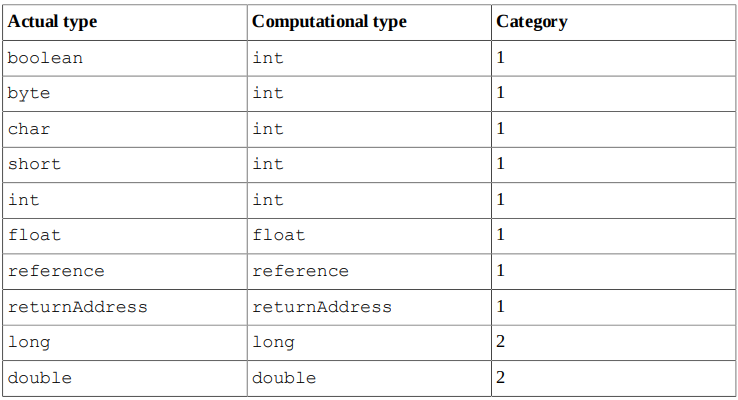
\includegraphics[width=400px]{images/2_JVM/computational_types.png}
    \caption{Computational types}
\end{figure}

\subsection{Practical examples}

\subsubsection{Types, branching and non-orthogonality}
The following code:
\begin{verbatim}
void spin() {
    int i;
    for (i = 0; i < 100; i++) {
        ; // Loop body is empty
    }
} 
\end{verbatim}
gets compiled to:
\begin{verbatim}
0 iconst_0      // push int constant 0 to stack
1 istore_1      // pop value from stack to local var 1
2 goto 8        // jump to line 8
5 iinc 1 1      // increment local var 1 by 1
8 iload_1       // push to stack local var 1
9 bipush 100    // push to stack int constant 100
11 if_icmplt 5  // compare values on stack, jump to 5 if first less than second
14 return       // return void when done
\end{verbatim}

Let's see for example some differences with double usage:
\begin{verbatim}
void spin() {
    double i;
    for (i = 0.0; i < 100.0; i++) {
        ; // Loop body is empty
    }
} 
\end{verbatim}
gets compiled to:
\begin{verbatim}
0 dconst_0      // push double constant 0.0
1 dstore_1      // store into local variables 1 and 2 (since double is 64 bit)
2 goto 9        // jump to line 9
5 dload_1       // push local variables 1 and 2
6 dconst_1      // push double constant 1.0
7 dadd          // add since there is no dinc instruction
8 dstore_1      // store result in local variables 1 and 2
9 dload_1       // push local variables 1 and 2
10 ldc2_w #4    // push double constant 100.0
13 dcmpg        // there is no if_dcmplt instruction
14 iflt 5       // compare and loop if less than(i < 100.0)
17 return       // return void when done
\end{verbatim}

So we can say that:
\begin{itemize}
    \item small int constants can be pushed to the stack directly with \verb|bipush n|;
    \item large int constant must be taken from the constant pool with \verb|ldc #n|;
    \item long constant must be taken from the constant pool with \verb|ldc2_w #n|;
    \item and more...
\end{itemize}

\subsubsection{Parameter passing}
\begin{verbatim}
int addTwo(int i, int j) {
    return i + j;
}
\end{verbatim}
gets compiled to:
\begin{verbatim}
0 iload_1       // Push value of local variable 1 (i)
1 iload_2       // Push value of local variable 2 (j)
2 iadd          // Add; leave int result on operand stack
3 ireturn       // Return int result
\end{verbatim}
because the parameters are stored inside the local variable array and the return value is taken from the stack.

NB: local variable 0 is used to store the reference to the \verb|this| value, so if the function is static the parameters would have been stored in 0 and 1.

\subsubsection{Invoking methods and functions}
\begin{verbatim}
int add12and13() {
    return addTwo(12, 13);
}
\end{verbatim}
gets compiled to:
\begin{verbatim}
0 aload_0           // Push local variable 0 (this)
1 bipush 12         // Push int constant 12
3 bipush 13         // Push int constant 13
5 invokevirtual #4  // Method Example.addtwo(II)I
8 ireturn           // Return int on top of operand stack;
\end{verbatim}
in practice the instruction \verb|invokevirtual #n| causes the allocation of a new frame, pops the arguments from the caller stack and places them inside the callee local variable array (along with \verb|this| reference in position 0), then change the program counter to the function address.
If the method has never called before the resolution of the symbolic link is performed.
In the end the opcode \verb|ireturn| pops the value from the top of the calle stack and places it onto the caller stack, destroys the frame and gets the control back to the caller.

There exists various method invocation:
\begin{itemize}
    \item \verb|invokevirtual|: used in order to call class methods on object instance;

    \item \verb|invokestatic|: used for calling static methods, arguments are copied to local vars starting from position 0 since there is no \verb|this| reference to pass; 

    \item \verb|invokespecial|: used for calling constructors (which are not dynamically dispatched), private methods or superclass methods.
    Of course \verb|this| reference is always passed.

    \item \verb|invokeinterface|: is the same as \verb|invokevirtual| but is used when the called method is declared in an interface (because it requires a different kind of method lookup);

    \item \verb|invokedynamic|: it has been introduced in Java SE 7 to support dynamic typing, fundamental in lambdas implementation (more on that later).
\end{itemize}

\subsubsection{Dealing with objects}
\begin{verbatim}
Object create() {
    return new Object();
}
\end{verbatim}
gets compiled to:
\begin{verbatim}
0 new #1            // Class java.lang.Object
3 dup               // duplicates the top element from the stack
4 invokespecial #4  // Method java.lang.Object.<init>()V
7 areturn
\end{verbatim}
First the \verb|new #n| opcode is used in order to create on the heap the needed memory for the desired object type and to get a reference to it.
Then \verb|invokespecial #n| is used in order to call the \verb|<init>| method, which is one of the constructor of that class, passing as first argument the \verb|this| reference, of course.

To access object fields we have two special instructions:
\begin{verbatim}
void setIt(int value) {
    i = value;
}
int getIt() {
    return i;
}
\end{verbatim}
gets compiled into:
\begin{verbatim}
Method void setIt(int)
0 aload_0
1 iload_1
2 putfield #4 // Field Example.i I
5 return
Method int getIt()
0 aload_0
1 getfield #4 // Field Example.i I
4 ireturn
\end{verbatim}
so the opcode \verb|putfield #n| takes two arguments from the stack which are the reference to the instance and the value we want to write, and inside the opcode there is a reference in the constant pool which tells us which field of the object we want to access.
The opcode \verb|getfield #n| instead takes the reference to the object we want to access via stack and the reference to the constant pool for the field using the opcode itself.
Both instructions require the resolution of the symbolic reference in the constant pool, then computes the offset of the field inside the class and uses it to access the field in the \verb|this| object.

For static fields the mechanisms is similar but with the opcodes \verb|putstatic| and \verb|getstatic|.

\subsubsection{Dealing with arrays}
The following statements:
\begin{verbatim}
buffer = new int[bufsz];
buffer[10] = value;
value = buffer[11];
\end{verbatim}
are translated into:
\begin{verbatim}
...
6 iload_2       // push array size
7 newarray int  // create new array of int of specified size
...
10 aload_1      // push reference to array
11 bipush 10    // push position
13 iload_3      // push value to write
14 iastore      // perform array write
...
15 aload_1      // push reference to array
16 bipush 11    // push position
18 iaload       // perform array read
...
\end{verbatim}  

\subsubsection{Switches}
A switch statement can be compiled using two different opcodes:
\begin{verbatim}
int chooseNear(int i) {
    switch (i) {
        case 0: return 0;
        case 1: return 1;
        case 2: return 2;
        default: return -1;
}}
\end{verbatim}
can be compiled into:
\begin{verbatim}
0 iload_1
1 tableswitch 0 to 2:
    0: 28
    1: 30
    2: 32
    default:34
28 iconst_0
29 ireturn
30 iconst_1
31 ireturn
32 iconst_2
33 ireturn
34 iconst_m1
35 ireturn
\end{verbatim}
in which the \verb|tableswitch| uses the value pushed to the stack to directly access one of the specified branches (if in range, otherwise the default one).
So following the opcode there is some padding, then three 32 bit words specifying the default branch, the low and high values for the range, and in the end there is a table of $high-low+1$ 32 bit words specifying the offset of each branch.

Otherwise if the range is not compact like:
\begin{verbatim}
int chooseFar(int i) {
    switch (i) {
        case -100: return -1;
        case 0: return 0;
        case 100: return 1;
        default: return -1;
} }
\end{verbatim}
it can be compiled to:
\begin{verbatim}
0 iload_1
1 lookupswitch 3:
        -100: 36
        0: 38
        100: 40
    default: 42
36 iconst_m1
37 ireturn
38 iconst_0
39 ireturn
40 iconst_1
41 ireturn
42 iconst_m1
43 ireturn
\end{verbatim}
Each case is a pair $<$value,address$>$, cases are sorted so that you can binary search for the actual match.

NB: both switches instructions only supports int so every other type must be converted, which is easy for char, byte, short, etc but it's a little bit tricky for type like Strings or object which need to pass by an hash function.

\subsubsection{Exceptions}
\begin{verbatim}
void cantBeZero(int i) throws TestExc{
    if (i == 0) {
        throw new TestExc();
    }
}
\end{verbatim}
gets compiled into:
\begin{verbatim}
0 iload_1           // Push argument 1 (i)
1 ifne 12           // If i==0, allocate instance and throw
4 new #1            // Create instance of TestExc
7 dup               // duplicate reference on top of stack
8 invokespecial #7  // Method TestExc.<init>()V
11 athrow           // Second reference is thrown
12 return           // Never get here if we threw TestExc
\end{verbatim}
to throw a new exception we first need to allocate it using \verb|new #n|, build it calling a constructor, then to throw it we use \verb|athrow|.
That opcode looks in the method for a catch block for the thrown exception using the exception table, if it exists the stack is cleared and the control passes to it, otherwise the whole frame is discarded and the same exception is thrown on the caller.
Of course if no method catches the exception the thread is aborted.

To add an exception table to the method a try/catch/finally block needs to be added:
\begin{verbatim}
void catchOne() {
    try {
        tryItOut();
    } catch (TestExc e) {
        handleExc(e);
    }
}
\end{verbatim}
which gets compiled to:
\begin{verbatim}
0 aload_0           // Beginning of try block
1 invokevirtual #6  // Method Example.tryItOut()V
4 return            // End of try block; normal return
5 astore_1          // Store thrown value in local var 1
6 aload_0           // Push this
7 aload_1           // Push thrown value
8 invokevirtual #5  // Invoke handler method:
                    // Example.handleExc(LTestExc;)V
11 return           // Return after handling TestExc

Exception table:
From    To  Target  Type
0       4   5       Class TestExc
\end{verbatim}
the exception table says that if an exception gets thrown between line 0-4 and the exception is of type \verb|TestExc| then the handler code is at line 5.

\subsubsection{More}
There exists then more instructions for example:
\begin{itemize}
    \item \verb|monitorenter| and \verb|monitorexit|: used to handle synchronization;
    \item \verb|instanceof|: to verify instances;
    \item \verb|checkcast|: to check a cast operation;
    \item \verb|nop|.
\end{itemize}

\subsection{Limitations}
Since the class file structure has a specified format there exists some limitations:
\begin{itemize}
    \item the max number of entries inside the constant pool is 65535;
    \item the max number of fields, methods and direct superinterfaces is 65535;
    \item max number of local variables in the local variable array of a frame is 65535;
    \item max operand stack size is 65535;
    \item max number of parameters of a method is 255;
    \item max length of field and method names is 65535 characters;
    \item max number of dimensions in an array is 255.
\end{itemize}

\section{Exercises}
\subsection{Exercise 1}
Write a simple Java program JustCreate that in a very long loop creates at each iteration one object, discarding immediately any reference to it.
Every 1000 iterations the program must print the number of objects created since the beginning, and must pause for one second (use e.g. Thread.sleep()).
Inspect the program execution with VisualVM.

\begin{verbatim}
/**
 *
 * @author drw0if
 */
public class JustCreate {
    public static void main(String[] args) throws InterruptedException {
        while (true) {
            var tmp = new DummyClass();
            if (DummyClass.instance_counter % 1000 == 0) {
                System.out.println("Up to now: " + DummyClass.instance_counter);
                Thread.sleep(1000);

            }
        }
    }
}

class DummyClass {
    public static int instance_counter = 0;
    int dummy_data;

    DummyClass() {
        dummy_data = 0;
        instance_counter++;
    }
}
\end{verbatim}
Inspecting the program with VisualVM we can notice that the memory consumption increases for a while, then it drastically decreases, that's because the garbage collector frees he allocated memory but not unused.
So the program flow is an alternating between memory usage increasing and then a drop in the consumption, in a loop.

\subsection{Exercise 2}
As we have seen recently, the JVM has two instructions that can be used to compile a \verb|switch| statement: \verb|tableswitch| and \verb|lookupswitch|.
Taking inspiration from the examples seen at lesson, try to determine when your Java compiler uses \verb|tableswitch| and when it uses \verb|lookupswitch|.
Does this depend only on the distance between the smallest and the largest constants in the case clauses? Are other criteria considered as well?

It seems that the driving factor in the decision is the compactness of the elements inside the switch.
For example:
\begin{verbatim}
public void sparseSwitch(int x) {
    switch (x) {
        case 0:     break;
        case 20:    break;
        default:
    }
}

public void notSoSparseSwitch(int x) {
    switch (x) {
        case 0:     break;
        case 1:     break;
        case 2:     break;
        case 3:     break;
        case 4:     break;
        case 5:     break;
        case 10:    break;
        case 15:    break;
        case 20:    break;
        default:
    }
}
\end{verbatim}
the first one is compiled using lookupswitch and the second one with tableswitch but both have 20 as the distance between the largest and the smallest value in the switch, the actual difference is the sparseness.

\subsection{Exercise 3}
Run the program WrongQueue and inspect its behaviour using visualvm.
Can you explain the continuos growth of the heap? Find the code causing the bug and fix it.

Inspecting the execution of the program with VisualVM we can notice a continual increase in the heap size and usage:
\begin{figure}[H]
    \centering
    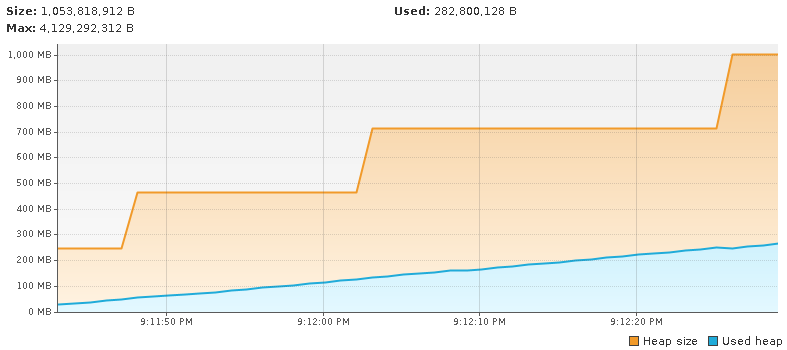
\includegraphics[width=400px]{images/2_JVM/WrongQueue.png}
    \caption{Heap usage in WrongQueue example program}
\end{figure}

That's because the garbage collector can't free the unused memory.
That issue is caused by the fact that the \verb|head| of the queue is never moved, so there always exists a reference to it and so since the object is reachable it never gets dropped.
That condition then spreads across all the elements of the queue so no node is dropped.

\subsection{Exercise 4}
During the last lesson, the lecturer claimed that when compiling a switch based on a String value, the Java compiler uses a hashing function for strings.
Also, if the hash value coincides with the hash of a string of a case clause, an additional comparison between the two string is performed.
Using javap, disassemble the compiled code to see if the lecturer is right.
Also, search in the Java or JVM Specification the precise place where this compilation scheme is prescribed.

So the following code:
\begin{verbatim}
switch ("asd") {
    case "aa":
        break;
    case "bb":
        break;
    default:
}
\end{verbatim}
gets compiled into:
\begin{verbatim}
...
6: invokevirtual #3     // Method java/lang/String.hashCode:()I
9: lookupswitch  {      // 2
            3104: 36
            3136: 50
         default: 61
    }
36: aload_1
37: ldc           #4    // String aa
39: invokevirtual #5    // Method java/lang/String.equals:(Ljava/lang/Object;)Z
42: ifeq          61
45: iconst_0
46: istore_2
47: goto          61
50: aload_1
51: ldc           #6    // String bb
53: invokevirtual #5    // Method java/lang/String.equals:(Ljava/lang/Object;)Z
56: ifeq          61
...
\end{verbatim}
so first the string gets hashed using \verb|hashCode| method, then the resulting value is used inside the switch case and if there is a match then th string is compared with the actual string inside the switch case using \verb|String.equals|.

\subsection{Exercise 5}
Run and inspect the program GCstrange using VisualVM, in particular check the evolution of the heap, the activity of the GC and the activity of the Finalizer thread.
Using GCstrange as a template, write a simple class that overrides the method finalize in order to estimate how many times the garbage collector is invoked.
Write a main to test this class.

\begin{verbatim}
import java.util.*;

class GCstrange {
    static List<GCstrange> dump = new LinkedList<>();
    static final int COUNT = 10000000;

    public static void main(String[] args) throws InterruptedException {
        GCstrange tmp = null;
        for (int i = 1; i < COUNT; i++) {
            if (i % (COUNT / 100) == 0) {
                System.out.println(i + " => " + dump.size());
                Thread.sleep(1000);
            }
            // creates a new instance
            tmp = new GCstrange();
            // the object is not reachable anymore
        }
    }

    public GCstrange() {}

    protected void finalize() {
        dump.add(this);
    }
}
\end{verbatim}
So we have an overriden \verb|finalize| method which saves a reference to the object inside a global list, so actually the garbage collector never frees anything.
\begin{figure}[H]
    \centering
    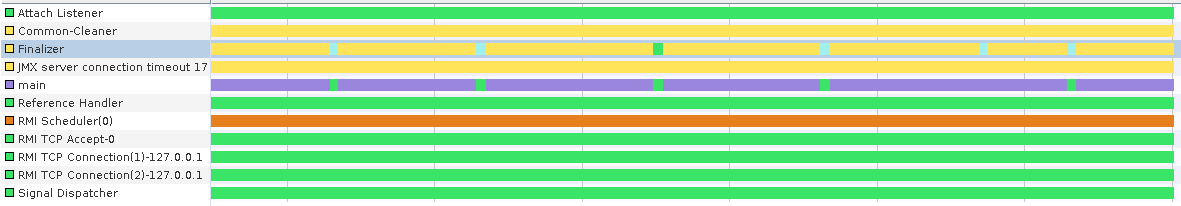
\includegraphics[width=430px]{images/2_JVM/GCStrange.png}
    \caption{VisualVM thread trace}
\end{figure}
The finalizer thread is almost always waiting except in some time slots in which it monitors (the blue one) and in execution in just one time slot.

To gets notices when the garbage collector is in execution we can print a timestamp inside the finalize method, so let's override it:
\begin{verbatim}
...
static long last_call = 0;
...
protected void finalize(){
    long current_ts = System.currentTimeMillis();

    // Drop consecutive call
    if (current_ts - last_call > 100){
        System.out.println("GC called at: " + current_ts);
        last_call = current_ts;
    }
}
\end{verbatim}
an example output could be:
\begin{verbatim}
100000 => 0
200000 => 0
300000 => 0
400000 => 0
500000 => 0
GC called at: 1676496620593 for the: 1 time
GC called at: 1676496621681 for the: 68652 time
...
GC called at: 1676496623800 for the: 119314 time
...
GC called at: 1676496625909 for the: 171725 time
...
GC called at: 1676496628022 for the: 224141 time
...
GC called at: 1676496632259 for the: 276550 time
...
GC called at: 1676496682247 for the: 355154 time
6300000 => 0
GC called at: 1676496682348 for the: 375998 time
GC called at: 1676496682449 for the: 388887 time
GC called at: 1676496682550 for the: 396121 time
GC called at: 1676496682651 for the: 769887 time
6400000 => 0
6500000 => 0
6600000 => 0
GC called at: 1676496686508 for the: 1198712 time
6700000 => 0
GC called at: 1676496686609 for the: 1347507 time
6800000 => 0
GC called at: 1676496689155 for the: 1382190 time
...
\end{verbatim}
